\documentclass[../main.tex]{subfiles}

\begin{document}
Después del análisis del estado del arte, se pueden obtener los requisitos necesarios para desarrollar el software de este proyecto.

Para poder completar los objetivos descritos en la sección \ref{Objectives}, es imprescindible una estructura de datos que permita almacenar toda la información necesaria sobre el laberinto de forma que sea accesible en todo momento. Con este fin, la estructura de datos que se ha escogido es un grafo ya que, como se explicará posteriormente, se adapta muy bien al concepto de este proyecto.

La prioridad principal en todo momento será la integridad del usuario, por lo que al generar las secciones hay que tener en cuenta todos los movimientos que este pudiera realizar para que siempre se encuentre dentro de los límites del espacio de trabajo. Teniendo esto en cuenta, el algoritmo que genera las secciones procedimentalmente debe funcionar de manera que las características de los laberintos sean completamente aleatorias, aumentando así la variedad. 

Como lo que se busca generar son laberintos que el usuario pueda explorar y en los que pueda perderse, si se cumplen las condiciones necesarias para ello, las secciones deben tener una probabilidad de crear caminos alternativos, es decir, ramificaciones que no lleven al final. 

Además, dado que el efecto de portal que se ha utilizado supone una carga computacional considerable y los laberintos que se generan son de longitud potencialmente infinita, solo se deben cargar las secciones del laberinto que sean necesarias para la posición actual del usuario, para aumentar así la eficiencia y evitar problemas. Esto es posible gracias al motor gráfico Unity, que proporciona los dos componentes necesarios para renderizar texturas, el Shader y el Material, y a los datos que se obtienen del grafo generado.

Para poder satisfacer estos requisitos, se ha dividido el proceso de generación del laberinto en 3 pasos, que deben hacerse secuencialmente y en un orden específico:

\begin{itemize}
    \item 1. Generar las características tanto del laberinto como de sus diferentes secciones procedimentalmente.
    \item 2. Renderizar las secciones necesarias, es decir, las que deben estar para que el usuario pueda mirar a través de cualquier portal y ver la sección conectada.
    \item 3. Conectar los portales coherentemente, según lo indique la estructura de datos generada en el paso 1.
\end{itemize}

Esta división es necesaria ya que uno de los requisitos es generar las secciones dinámicamente, mientras el usuario explora el entorno. Los portales deben conectarse siempre después de renderizarse, ya que antes del renderizado no existen y por lo tanto sería imposible su conexión.

Una vez planteados estos requisitos, a continuación se detalla el desarrollo del proyecto estructuradamente, siguiendo los objetivos a alcanzar.

\section{Migración a Unity XR}

Como se explica en la sección \ref{UnityXR_Section}, Unity XR es un sistema que busca unificar los conceptos de realidad virtual, aumentada y mixta. 

Una de sus principales ventajas es que permite a los desarrolladores crear software con implementaciones genéricas, de forma que se maximiza el número de dispositivos en los que se pueden ejecutar las aplicaciones sin necesidad de implementaciones específicas para cada uno. Esto significa que si en el futuro otra empresa desarrollara su Plug-in y lo integrase en Unity, sus dispositivos podrían ejecutar proyectos desarrollados con el sistema XR sin problema.

Por estos beneficios y funcionalidades, se ha decidido migrar el sistema de realidad virtual de forma que se pasa de utilizar la API de Oculus a utilizar Unity XR.

El primer paso para poder utilizar el nuevo sistema, tras añadir el paquete al proyecto, es refactorizar el código de manera que se utilicen las funciones de la API de Unity en vez de las de oculus. En la mayor parte de los casos esto solo es necesario cuando se tiene que acceder a la información del dispositivo, como la resolución de las pantallas de cada ojo y otros datos que son fundamentales para que se pueda crear la textura de los portales.

Una vez se ha adaptado el código, el siguiente paso es reemplazar el OVR de Oculus, que es el objeto que contiene todo lo necesario para los dispositivos Oculus para enviar las imágenes correctamente a cada ojo. El OVR contiene tres cámaras, una para cada ojo y otra cámara general. Como en Unity no es posible modificar la componente Transform de las cámaras de los ojos, lo cual es necesario para teletransportarlos al cruzar el portal, cada una de ellas tiene un objeto padre vacío que será el que se manipula.

Unity XR proporciona un objeto llamado Room-Scale XR Rig, que es el equivalente al OVR Rig de Oculus. Como su nombre indica, el Room-Scale XR Rig utiliza como sistema de movimiento Room Scale, explicado anteriormente. Uno de los principales cambios es que Oculus permite diferenciar fácilmente las cámaras de cada uno de los ojos mediante un atributo, mientras que en XR esto no es posible. Para solucionar esto, utilizaremos para cada cámara del objeto un Tracked Pose Driver.

Los Tracked Pose Driver son componentes que permiten actualizar la posición de un determinado dispositivo o una de sus cámaras, manipulando la componente Transform del GameObject. Este componente tiene un atributo que permite seleccionar qué movimiento se está siguiendo, el ojo izquierdo, derecho o la cámara principal. También se puede decidir el tipo de seguimiento que se hace, que para este proyecto es de tipo rotación y posición, es decir, 6 grados de libertad.

Finalmente, al objeto XR Rig se le ha asignado una cámara principal y un offset que representa la distancia al suelo. Además se le ha añadido un XR Interaction Manager, que es un componente que actúa como intermediario entre los objetos que interactúan en la escena. 

Después de este proceso tenemos un objeto que permite enviar a cualquier dispositivo compatible con Unity XR las imágenes a cada ojo correctamente, hacer un seguimiento y actualización de su posición e interactuar con objetos de la escena.

Sin embargo, al acceder a la información del dispositivo surge un problema ya que el módulo XR no se inicializa instantáneamente al ejecutar el proyecto, sino que necesita una cantidad muy pequeña de tiempo para hacerlo. Si se intenta acceder al dispositivo justo al ejecutar el proyecto, los valores que se reciben son incorrectos y por lo tanto el funcionamiento también. Esto supone un problema ya que en el proyecto se accede a estos valores en la función Start, que en Unity se ejecuta en el primer fotograma cuando el objeto que contiene el componente script está activo.

Para solucionarlo, se ha modificado el código para que estos accesos se hagan tras esperar una cantidad aproximada de 10 fotogramas, asegurando que se obtienen los datos correctos.

Como se ha mencionado anteriormente, el efecto de los portales supone una carga computacional significativa. En este proyecto, al conectar varias secciones utilizando dicho efecto, se pueden observar algunos fallos de rendimiento que llevan a peores experiencias al recorrer el laberinto.

Para solucionar esto, se han colocado los portales en una capa diferente en Unity, lo que permite desactivar la renderización de los objetos de dicha capa utilizando el atributo \textit{cullingMask} de sus cámaras auxiliares, que define los objetos que se renderizan según las capas en las que se encuentran. De esta forma se desactivan todos los portales a excepción de los que el usuario está viendo en tiempo real, evitando problemas de rendimiento y obteniendo una mejora en la sensación de presencia en el entorno.

Tras estos cambios y con la creación del nuevo objeto XR se ha terminado el proceso de migración del proyecto de la API de Oculus al sistema Unity XR.

\section{Diseño y Desarrollo del Generador de Laberintos Procedimental}

A continuación se explican todos los pasos realizados en el desarrollo del sistema de generación procedimental.

Se recuerda al lector que para todas las clases implementadas en el desarrollo del proyecto se ha utilizado el lenguaje C\#.

\subsection{Estructura de datos}

Antes de comenzar con el desarrollo del algoritmo procedimental, es necesario establecer una serie de clases que permitan almacenar la información que será necesaria para el correcto funcionamiento del proyecto. Estas serán finalmente tres clases complementarias que en su conjunto forman un grafo, y que controlan el laberinto, las diferentes secciones y sus conexiones respectivamente.

Para obtener un mejor entendimiento de cómo funcionan dichas clases, se explican a contuniación las razones por las que se elige un grafo para almacenar los laberintos.

La principal razón es que al estar el laberinto dividido en secciones interconectadas, se asemeja mucho a un grafo donde los nodos son las secciones y las conexiones entre estos, los portales. Para poder apreciar estas similitudes, se propone un ejemplo en la figura \ref{fig:Maze_Graph}.

Como se ve en la imagen, tenemos un laberinto generado aleatoriamente y almacenado en un grafo. Cada nodo de este grafo hace referencia a una sección diferente del laberinto y almacena todas sus características, y cada conexión entre dos nodos es en realidad la conexión de dos portales de secciones diferentes. Al estar dividido el laberinto en secciones, su disposición espacial es superpuesta en un mismo espacio físico, por lo que la distribución de este grafo está completamente superpuesta a uso práctico.

\begin{figure}[h!]
\centering
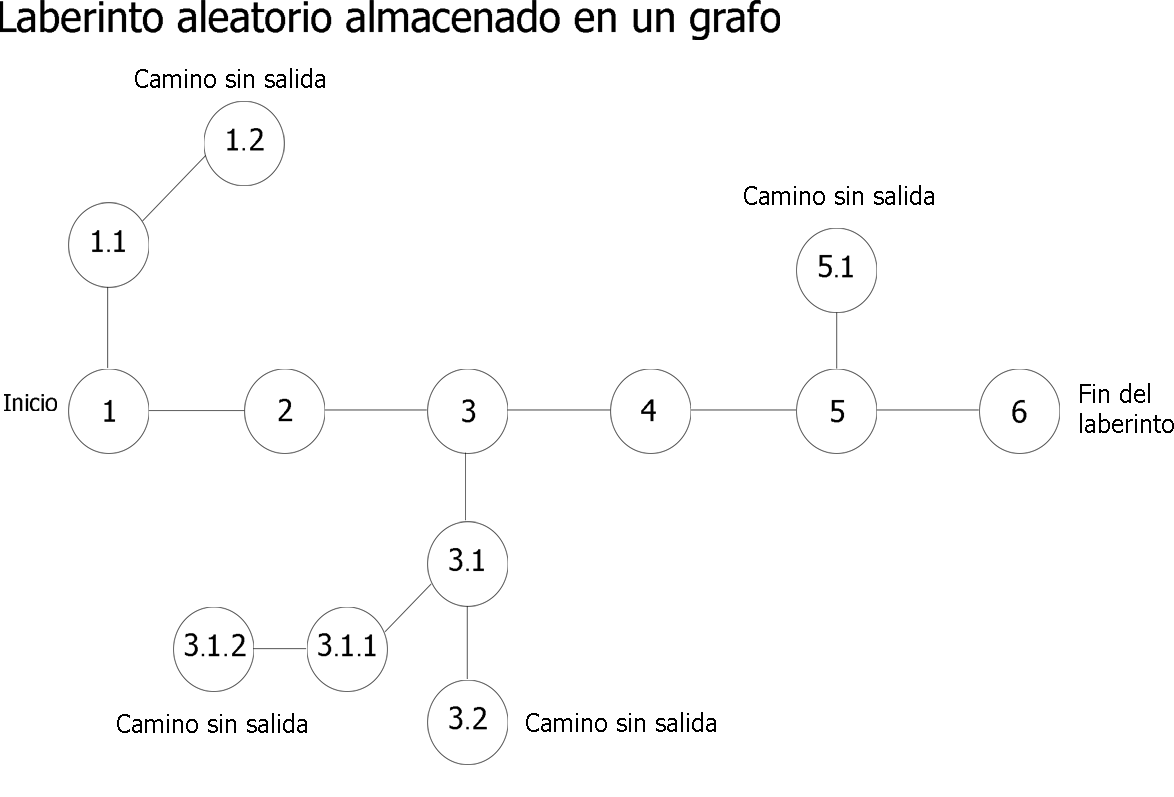
\includegraphics[width = 12cm, height = 8cm]{imagenes/Laberinto_Grafo.png}
\caption{Ejemplo de un laberinto aleatorio visto como un grafo.}
\label{fig:Maze_Graph}
\end{figure}

En el ejemplo, el camino 1 - 2 - 3 - 4 - 5 - 6 es el que lleva a la victoria, pero también existen caminos alternativos que llevan a ramificaciones del laberinto, que pueden tener recursivamente más ramificaciones dependiendo de la dificultad que se quiera conseguir, como se ve en el camino 1 - 2 - 3 - 3.1 - 3.1.1 - 3.1.2, que pasa por 2 ramificaciones diferentes además del camino principal. 

Esto significa que esta estructura de datos permite almacenar cualquier tipo de camino posible que pueda ser generado en el laberinto y, al ser el principal objetivo del proyecto generar laberintos de grandes dimensiones y varias ramificaciones diferentes, esto es un requisito imprescindible que se debe cumplir.

En la figura \ref{fig:Class_Diagram} se puede observar el diagrama de clases que define la estructura de datos que almacena los laberintos. Como se puede ver, los laberintos generados pueden tener de 0 a infinitas secciones, que están conectadas entre ellas. Estas conexiones también quedan guardadas en la clase Graph para que puedan ser accedidas en todo momento.

\begin{figure}[h!]
\hspace{-2.75cm}
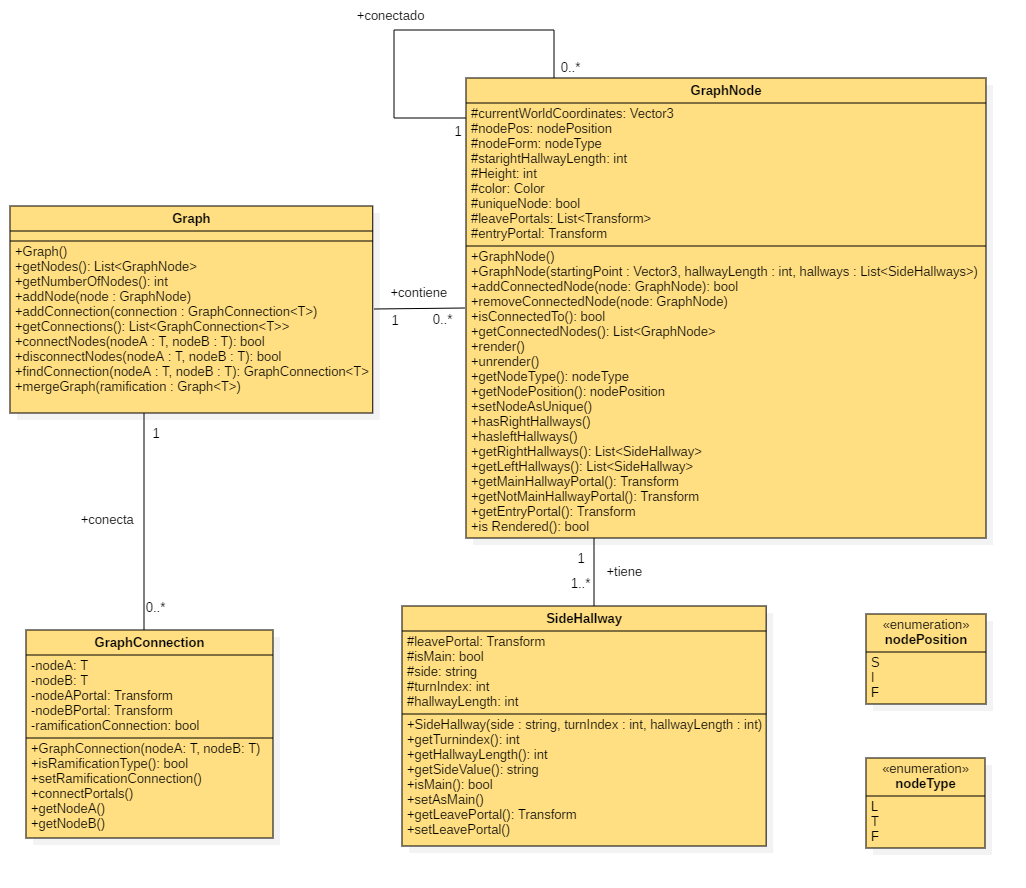
\includegraphics[width=1.5\textwidth, height = 17cm]{imagenes/Class_Diagram_TFG.png}
\caption{Diagrama de clases del grafo que almacena los laberintos generados}
\label{fig:Class_Diagram}
\end{figure}

Cada una de estas clases tiene una función principal y unos atributos y métodos que permiten que la pueda llevar a cabo, y que se explican más adelante.

A continuación se explican las funcionalidades que proporcionan estas clases, las conexiones entre ellas y cómo funcionan.

\subsubsection{Control del laberinto como conjunto: clase Graph}

La clase Graph supone la base del resto de clases y algoritmos utilizados en este Trabajo de Fin de Grado. Es la encargada de almacenar la información del laberinto entendido como un conjunto ya que permite almacenar tanto los nodos que forman el laberinto como las conexiones entre ellos.

Esta clase es genérica y está basada completamente en algoritmos sobre grafos, por lo que no implementa métodos específicos para la generación de laberintos. Su principal funcionalidad es la obtención de datos sobre las diferentes generaciones, permite saber el estado actual de la conexión entre cualquier par de nodos, así como conectarlos y desconectarlos, y también permite añadir nuevos nodos o saber el número total de estos. 
Conectar nodos desde esta clase no conecta los portales de las secciones, simplemente guarda las referencias necesarias en la estructura de datos para que puedan ser utilizadas posteriormente.

Por este motivo, esta clase tiene los siguientes atributos, donde T es genérico:

\begin{itemize}
    \item[$\blacksquare$] \textbf{protected List$<$GraphNode$>$ nodes:} lista que almacena todos los nodos que contiene el grafo.
    \item[$\blacksquare$] \textbf{protected List$<$GraphConnection$<$T$>$ $>$ connections:} lista que almacena todas las conexiones existentes entre los nodos del grafo
\end{itemize}

Además de estas funcionalidades, otra de las principales razones por la que se ha creado esta clase es para investigaciones futuras, de manera que se tenga control absoluto sobre el grafo y se pueda manejar como sea necesario, de la manera más flexible posible.

\subsubsection{Control de las secciones del laberinto: clase GraphNode}

Una vez explicada la clase Graph el siguiente paso es la clase GraphNode, que controla cada una de las secciones del laberinto por separado y almacena todos sus datos y características. 

Para poder comprender el funcionamiento de esta clase, primero es necesario entender qué características tienen las secciones del laberinto y cómo se manipulan. En primer lugar, todo el laberinto está formado por polígonos cuadrados de $1m^2$, rotados y posicionados según es necesario. Todas las secciones tienen un pasillo principal, cuya longitud mínima es 2 metros, y una lista de pasillos laterales tanto a la izquierda como a la derecha. 

Con la finalidad de evitar generar laberintos demasiado complicados, en este proyecto se ha limitado el número de pasillos laterales a un máximo de 2, pero la implementación permite añadir los que sean necesarios para investigaciones futuras. Por lo tanto, en este proyecto diferenciamos 3 formas distintas que una sección puede tener, en forma de L, T o F.

En la figura \ref{fig:Node_Types} se pueden ver tres secciones diferentes desde una perspectiva vertical. La forma más básica es la que tiene la sección A, que tiene un solo pasillo lateral, por lo que no da lugar a ninguna ramificación. Las dos formas restantes, tanto la que tiene la sección B como la C, implican la creación de una nueva ramificación en el laberinto. Los nodos en forma de T como los de la sección B tienen un pasillo a cada lado que jamás pueden estar en el mismo punto y deben estar separados por al menos 2 metros, es decir, desde dentro de uno de los pasillos debe ser imposible ver el interior del otro. Por último, los nodos en forma de F tienen dos pasillos laterales, ambos en el mismo lado, y pueden crearse en cualquier punto del pasillo, aunque nunca en el mismo punto. Si los pasillos están contiguos, la pared que los separa tiene un grosor menor, para evitar problemas de visualización del portal.

\begin{figure}[h!]
\centering
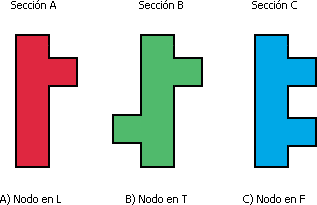
\includegraphics[width=9cm, height=5.5cm]{imagenes/NodeTypes.png}
\caption{Posibles formas de las secciones del laberinto.}
\label{fig:Node_Types}
\end{figure}

Toda la información sobre los pasillos laterales se encuentra en la clase sideHallway, que solo es utilizada por la clase GraphNode. La principal funcionalidad de esta clase es almacenar las características de los pasillos laterales, facilitando mucho el desarrollo y permitiendo seguir un proceso organizado. Para entender esta clase, a continuación se exponen sus atributos:

\begin{itemize}
    \item[$\blacksquare$] \textbf{protected Transform leavePortal:} componente Transform del portal de salida del pasillo lateral actual. Si es null, significa que en este pasillo se ha llegado al final, ya sea una ramificación o no.
    \item[$\blacksquare$] \textbf{protected string side:} indica el lado hacia el que se instancia el pasillo lateral. Si es "right" significa que es un pasillo lateral derecho, si es "left" significa que es un pasillo lateral izquierdo.
    \item[$\blacksquare$] \textbf{protected int turnIndex:} entero que indica en qué punto del pasillo principal aparece este pasillo lateral. Por ejemplo, si turnIndex es 4, significa que este pasillo se instancia a 4m del inicio del pasillo principal.
    \item[$\blacksquare$] \textbf{protected int hallwayLength:} entero que indica la longitud de este pasillo lateral.
    \item[$\blacksquare$] \textbf{protected bool ismain:} booleano que indica si este pasillo corresponde al camino principal actual o no. El camino principal se refiere al camino lineal que sigue el laberinto, si aparece un pasillo lateral que crea una nueva ramificación entonces ismain será false, en cualquier otro caso será true.
\end{itemize}

Los métodos que implementa esta clase sirven para acceder a estos datos o para asignar algunas variables como leavePortal. Es importante saber que esta clase permite la conexión con otros nodos, aunque esta se guarda simplemente como una referencia, para que quede constancia en todo momento, pero nunca permite realizar las conexiones entre los portales.



Una vez comprendidas las características de una sección del laberinto y cómo se almacenan los datos de los pasillos laterales, es más sencillo comprender el funcionamiento de la clase GraphNode. Esta es una de las clases clave del proyecto, y al contrario que la clase Graph, aunque se puede utilizar para crear nodos vacíos, su principal funcionalidad es la de crear nodos que almacenen las características de las secciones del laberinto y renderizarlas. Por esta razón, implementa distintos métodos que son necesarios para satisfacer los objetivos, principalmente para dar acceso a información importante sobre las secciones o para dar valores a algunos atributos específicos, que se utilizan más adelante al diseñar el algoritmo procedimental de generación del laberinto. 

Esta clase utiliza dos atributos de tipo enumeración, uno que controla la forma del nodo (L,T o F) y otro que controla la posición del nodo en el grafo (S,I,F). Este último diferencia entre nodo inicial, que es el primer nodo del laberinto, nodo intermedio, que son todos los nodos que tienen otros nodos delante y detrás, y nodo final, que son todos los nodos en los que se llega al fin, ya sea una ramificación o no.

Para comprender su funcionamiento al completo, se detallan todos sus atributos a continuación:

\begin{itemize}
    \item[$\blacksquare$] \textbf{protected List$<$GraphNode$>$ connectedNodes:} lista que contiene la referencia a todos los nodos con los que este nodo está conectado. Esta lista sirve solo para almacenar referencias y no crea ninguna conexión entre los nodos.
    \item[$\blacksquare$] \textbf{protected int straightHallwayLength:} entero que indica la longitud del pasillo principal de esta sección.
    \item[$\blacksquare$] \textbf{protected List$<$SideHallway$>$ rightHallways:} lista de pasillos laterales derechos de la sección actual.
    \item[$\blacksquare$] \textbf{protected List$<$SideHallway$>$ leftHallways:} lista de pasillos laterales izquierdos de la sección actual.
    \item[$\blacksquare$] \textbf{protected Transform entryPortal:} componente Transform del portal de entrada de esta sección del laberinto. Es único dado que una sección del laberinto solo puede ser accedida por un único portal.
    \item[$\blacksquare$] \textbf{protected List$<$Transform$>$ leavePortals:} lista que contiene los compo- nentes Transform de los portales de salida de esta sección del laberinto. A diferencia del portal de entrada debe ser una lista dado que para crear ramificaciones tiene que haber más de un camino y, por lo tanto, más de un portal de salida. El número de componentes de esta lista debe ser igual al número de pasillos laterales, ya que cada portal de salida corresponde a un pasillo lateral.
    \item[$\blacksquare$] \textbf{protected Vector3 currentWorldCoordinates:} coordenadas (x,y,z) iniciales del nodo. Son necesarias para renderizar el nodo en la posición adecuada.
    \item[$\blacksquare$] \textbf{protected int height:} entero que indica la altura en metros de esta sección.
    \item[$\blacksquare$] \textbf{protected Color color:} especifica el color que tiene la sección.
    \item[$\blacksquare$] \textbf{protected nodePosition nodePos:} atributo de tipo enumeración que indica la posición del nodo dentro del grafo. Los posibles valores son S (nodo inicial), I (nodo intermedio) y F (nodo final).
    \item[$\blacksquare$] \textbf{protected nodeType nodeForm:} atributo de tipo enumeración que especifica la forma de esta sección. Las posibles formas que puede tener un nodo, como se ha explicado anteriormente, son en forma de L, T o F.
    \item[$\blacksquare$] \textbf{protected bool uniqueNode:} booleano que sirve para indicar si esta sección es la única del camino desde el inicio del laberinto hasta el final.
    \item[$\blacksquare$] \textbf{protected GameObject parent:} referencia al objeto padre que agrupa todos los componentes de este nodo.
    \item[$\blacksquare$] \textbf{protected Object portal:} referencia al objeto portal de Unity, que se utiliza para poder instanciarlo desde código.
\end{itemize}

La clase dispone de 2 constructores, un constructor general que permite crear un nodo vacío, que simplemente tiene una lista de nodos conectados también vacía, y un segundo que, a partir del punto de inicio, la longitud del pasillo principal, las listas de pasillos laterales y la posición del nodo, permite crear los datos de una sección del laberinto. Estos constructores se han diseñado utilizando el concepto de sobrecarga. La sobrecarga de constructores permite definir más de un constructor o método con el mismo nombre, con la condición de que no puede haber dos de ellos con el mismo número y tipo de parámetros \cite{Sobrecarga_Constructores}. Esto permite llevar a cabo una tarea de distintas maneras, en este caso crear un nodo vacío o con las características de la sección del laberinto, dependiendo de qué sea necesario.

La sobrecarga de constructores es un concepto muy utilizado en la programación orientada a objetos, y permite diseñar clases desde una perspectiva más genérica.

Una vez están almacenadas las características de los nodos del grafo y sus conexiones, se puede renderizar cualquier nodo a partir de estos datos. El procedimiento que se utiliza para la renderización se explica más adelante.

\subsubsection{Control de las conexiones del laberinto : GraphConnection$<$T$>$}

Las clases explicadas anteriormente crean tanto las conexiones entre los nodos como los portales que interconectan las secciones. La clase GraphConnection sirve para que dichas conexiones aparezcan representadas en el grafo para que se puedan manipular o consultar correctamente.

Al igual que la clase Graph, esta clase es genérica. Su funcionamiento es muy simple, ya que su uso es únicamente almacenar la información de la conexión entre dos nodos. Además permite conectar los portales de las secciones que tengan una conexión existente, siempre después de haberlas renderizado, lo que permite que el usuario pueda pasar de una a otra.

Para conseguir lo descrito anteriormente, la clase tiene los siguientes atributos:

\begin{itemize}
    \item[$\blacksquare$] \textbf{private T nodeA:} referencia al nodo del que parte la conexión.
    \item[$\blacksquare$] \textbf{private T nodeB:} referencia al nodo al que llega la conexión.
    \item[$\blacksquare$] \textbf{private Transform nodeAPortal:} componente Transform del portal de salida del nodoA que se quiere conectar.
    \item[$\blacksquare$] \textbf{private Transform nodeBPortal:} componente Transform del portal de entrada del nodoB que se quiere conectar.
    \item[$\blacksquare$] \textbf{private bool ramificationConnection:} booleano que indica si la conexión actual es de inicio de ramificación. Si es true, el portal de salida nodeAPortal que se elige es el no principal y si es false el que se elige es el principal.
\end{itemize}

La clase GraphConnection es completamente necesaria para mantener la integridad del grafo como conjunto y tener control absoluto sobre sus conexiones en todo momento ya que sin ella, sería imposible para el usuario navegar entre secciones

\subsection{Renderización de las secciones del laberinto}

Como se explica previamente, a partir de las características de las secciones se generan los objetos tridimensionales que las forman. En este apartado se explica paso a paso el proceso que se sigue para conseguir este objetivo.

\subsubsection{Renderización de Mesh desde código}

Como se explica en la sección \ref{Unity_Rendering}, para poder renderizar en Unity, es necesario utilizar un Mesh, que es el componente que define la forma de un objeto en tres dimensiones. Funciona como una red de puntos o vértices, donde las líneas invisibles que los conectan forman triángulos que le dan forma al objeto. 

\begin{figure}[h!]
\centering
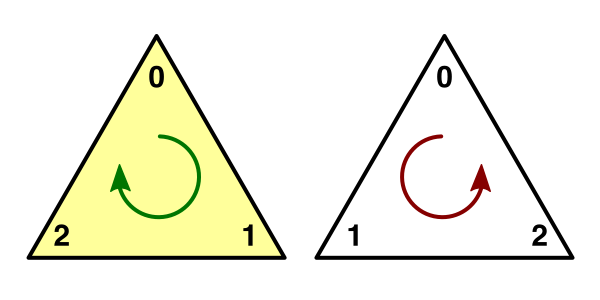
\includegraphics[width=9.25cm, height=5cm]{imagenes/Triangle_Render.png}
\caption{Orientación de la cara de un polígono según la orientación de la conexión de sus vértices. Fuente:\cite{Unity_Render}}
\label{fig:Triangle_Render}
\end{figure}

Además de la forma, es necesario saber qué orientación tienen las caras del objeto en cuestión ya que en Unity será la única que se renderize para aumentar la eficiencia. Para definir esto, es necesario definir un vector que contenga las coordenadas de los vértices del polígono, y otro que defina el orden en el que se conectan. Este último, además de definir qué vértices se conectan, también especifica el orden con el que lo hacen y, consecuentemente, la orientación de su superficie. Tal y como se ve en la figura \ref{fig:Triangle_Render}, si los vértices se conectan en el sentido de las agujas del reloj, en Unity significa que está de frente, mientras que si se conectan en sentido contrario a las agujas del reloj, es la cara contraria la que se renderiza.

Con estos datos ya es posible crear triángulos con las características necesarias y, a partir de estos, cualquier polígono. 

Para crear las diferentes secciones, como se ha mencionado anteriormente, se han utilizado cuadriláteros, de manera que podamos crear la base de $1m^2$ que sirve para generar la sección. Para poder crear una cara de este polígono es suficiente con dos triángulos.

Dichos triángulos deben estar posicionados de forma que estén contiguos en la escena, y la orientación de sus caras debe ser la misma, como se ve en la figura \ref{fig:Quad_Render}.

\begin{figure}[h!]
\centering
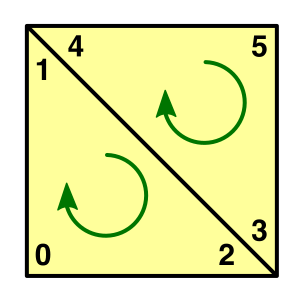
\includegraphics[width=5cm, height=5cm]{imagenes/Quad_Render.png}
\caption{Renderización de un cuadrilátero a partir de dos triángulos. Fuente:\cite{Unity_Render}}
\label{fig:Quad_Render}
\end{figure}

Sin embargo, el objeto no está terminado aún ya que aún no se le ha asignado ninguna textura. Para el desarrollo de este proyecto se han utilizado texturas básicas proporcionadas por Unity sobre las que más tarde se modifican algunos parámetros, y que se añadirán a la componente Mesh de los objetos.

Teniendo todos los datos del polígono, se crea en la escena un objeto vacío por cada uno de ellos, y se le añade desde código la componente Mesh con dichos datos. Para agregar aleatoriedad a la generación de secciones, en el constructor se asigna a la sección un color aleatorio dentro de un rango, que es el que se le asigna a cada uno de los polígonos que se instancian posteriormente, de forma que cada sección tenga un color aleatorio pero los polígonos que las componen tengan el mismo. También se han calculado las normales mediante la API de Unity, para que la refracción de la luz sobre el objeto quede lo más realista posible.

Por último, para mantener un orden y estructurar los objetos de la escena, cada polígono que se instancia y que forma la sección se ha asignado cómo hijo de un objeto padre que tiene asignada cada una de ellas.

En este punto es posible crear los polígonos de $1m^2$ en cualquier punto de la escena y con cualquier rotación y se ha hecho uso de esto para generar los suelos, paredes y techos de las secciones. A continuación se explica cómo se aplica este proceso para la renderización de las secciones de los laberintos.

\subsubsection{Renderización del Mesh de las secciones del laberinto desde código}

Para generar el pasillo principal, es suficiente con instanciar un objeto por cada metro de longitud que tiene, es decir, si un pasillo mide 5 metros, se instancian 5 objetos contiguos, avanzando positivamente en el eje de las z (Que transformándolo a un plano bidimensional correspondería con el eje de las y).

Para los pasillos laterales se procede de la misma manera, pero si el pasillo es hacia la izquierda se avanza negativamente por el eje de las x, y si es hacia la derecha se avanza positivamente por el mismo. Además, los pasillos laterales deben comenzar donde se especifique, es decir, si un pasillo lateral comienza en el índice 5, quiere decir que debe instanciarse a partir del quinto objeto del pasillo principal.

\begin{figure}[h!]
\hspace{-1.25cm}
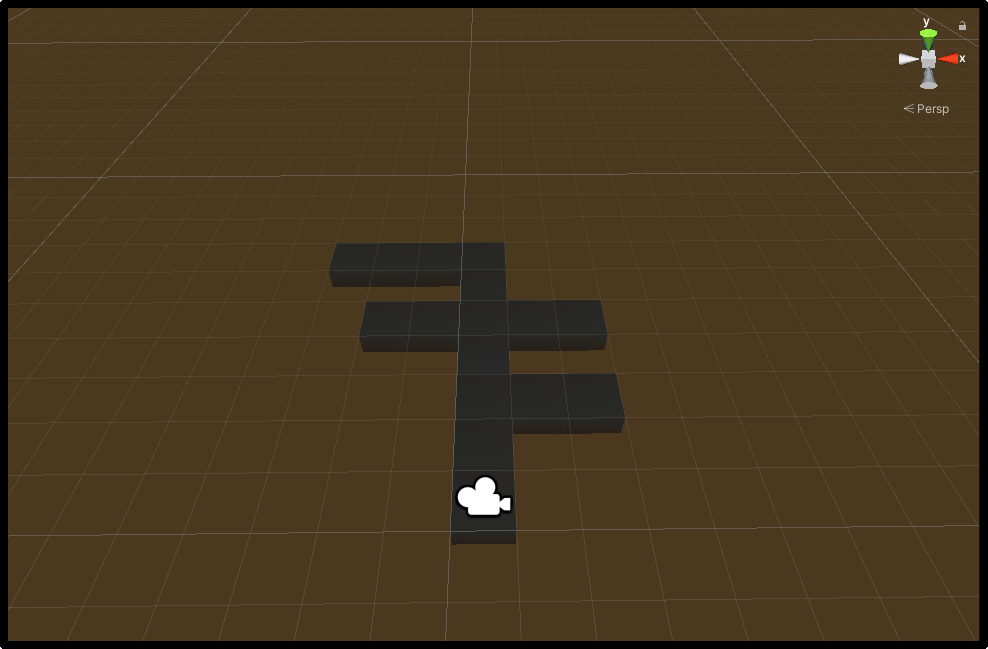
\includegraphics[width=15cm, height=10cm]{imagenes/Floor_Node_Example.png}
\caption{Ejemplo de renderización del suelo de una sección del laberinto.}
\label{fig:Floor_Unity_Example}
\end{figure}

En el ejemplo de la figura \ref{fig:Floor_Unity_Example}, se puede observar este proceso sobre una sección cuyo pasillo principal mide 7 metros, con dos pasillos laterales derechos de 2 metros, y dos pasillos laterales izquierdos de 2 y 3 metros respectivamente. Los pasillos derechos comienzan en los índices 3 y 5, mientras que los izquierdos comienzan en los índices 5 y 7.

Con este sistema, ya es posible generar todas las secciones del laberinto mostrando su información principal, pero para conseguir el laberinto al completo es necesario renderizar también las paredes y techos para mantener la integridad del entorno no euclidiano y los portales para que el usuario pueda moverse entre secciones.

Para representar las paredes en la escena se han utilizado los mismos polígonos que en el suelo, pero rotados de manera que queden en vertical. Como pueden ser necesarias distintas rotaciones dependiendo de si pertenecen al pasillo principal o a uno de los pasillos laterales, se ha creado un método que permite generar una pared con cualquier rotación posible, en la posición deseada. 

La altura de las secciones del laberinto determina cuántos de estos objetos se deben renderizar contiguos verticalmente para crear la pared como conjunto. Un ejemplo sería el que se ve en la figura \ref{fig:Wall_Unity_Example} si la altura es 5, significa que la pared generada serán 5 polígonos con la posición y rotación especificadas separados verticalmente 1 metro para que estén contiguos y, en conjunto, sean una pared de 5 metros de alto y 1 metro de ancho. Esta altura es la misma para todas las paredes que se generan, y para generarlas todas es suficiente con repetir este proceso con las posiciones y rotaciones adecuadas, dependiendo del pasillo del que se trate.

\begin{figure}[h!]
\hspace{-1.5cm}
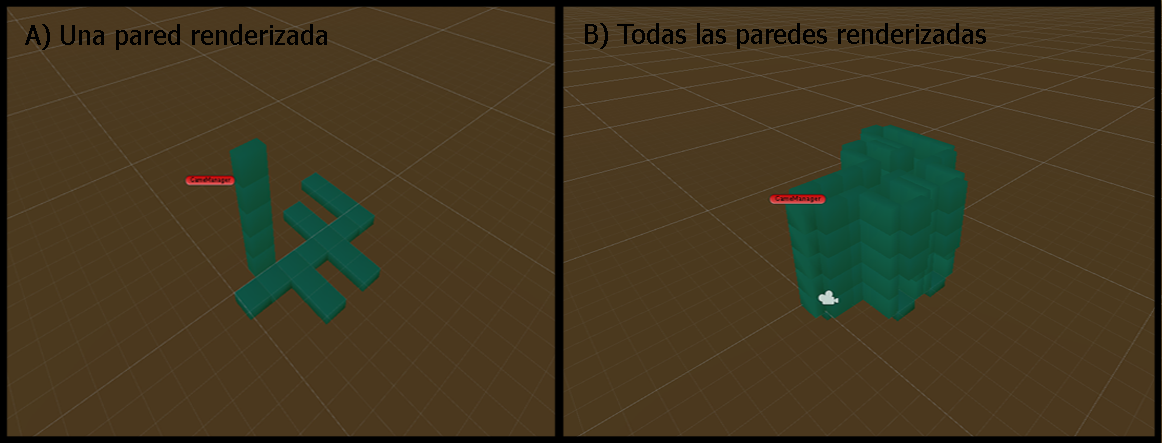
\includegraphics[width=16cm, height=8cm]{imagenes/Wall_Rendering.png}
\caption{Ejemplo de renderización de las paredes de una sección del laberinto. (A) Una pared renderizada. (B) Todas las paredes renderizadas.}
\label{fig:Wall_Unity_Example}
\end{figure}

Si el pasillo es el principal, se debe dejar abierto el camino hacia los pasillos laterales que se hayan instanciado. También se debe recordar que, para conectar las secciones, se utilizan unos portales, que para este proyecto serán de 3 metros de alto. Estos portales, cuando son necesarios, se generan al principio de la sección y al final de los pasillos laterales. Por lo tanto, al final los pasillos laterales que se conecten mediante un portal, se debe dejar espacio suficiente para instanciarlo, generando solo las paredes que estén por encima de este. Se sigue el mismo procedimiento para el comienzo de las secciones.

En este proyecto se ha diferenciado entre portales de salida, que son los portales que se crean al final de los pasillos laterales, y pasillos de entrada, que son los que se crean al comienzo de la sección.

Sin embargo, existen excepciones en las que no son necesarios los portales. Estas son las secciones en las que termina el laberinto o una ramificación (Nodos cuya posición es F), y la primera sección del laberinto (Nodo cuya posición es S). En estos casos, que son los nodos cuya posición no es intermedia, se procede de la siguiente manera:

\begin{itemize}
    \item En el primer caso, si es un nodo sin ramificaciones, basta con no generar el portal y simplemente crear las paredes. Si es una sección con forma de T o F, es necesario identificar el pasillo principal para que en dicho pasillo no se genere el portal y en su lugar se cierre con paredes. Si la sección tiene varios pasillos laterales, pertenece al camino principal, y es la última del camino, significa que esta sección es la sección final del laberinto, por lo tanto, se cierran todos los pasillos laterales con paredes.
    \item En el segundo caso, al ser la primera sección, nunca se genera el portal de entrada a la sección. Además, si este nodo es el único del laberinto, también se cierran los portales de salida con paredes.
\end{itemize}


Una vez entendida la lógica utilizada para generar las paredes de las diferentes secciones del laberinto, hay que controlar algunos casos específicos para evitar que se superpongan unas sobre otras, ya que esto genera problemas de rendimiento.

Este problema surge principalmente en los giros de 90º que se crean al generar un pasillo lateral, ya que siguiendo la lógica explicada anteriormente, las paredes colisionan justo en la esquina, como se ve en la figura \ref{fig:Wall_Overlapping}. La solución es mover las paredes en el eje de las x, dependiendo del pasillo lateral del que se trate, una cantidad igual al grosor del objeto, de manera que estén contiguos pero no se superpongan.

Si el pasillo lateral es hacia la izquierda, las paredes se desplazan hacia la izquierda, y si el pasillo lateral es hacia la derecha, se desplazan  hacia la derecha.

El único caso en el que esto no es un problema es cuando el pasillo lateral se genera contiguo al primer o último polígono del pasillo principal, en todos los demás casos es necesario desplazar las paredes del pasillo lateral.

La última excepción ocurre cuando una sección en F tiene 2 pasillos laterales contiguos. En este caso la pared que los separa se hace de un grosor mínimo para evitar problemas de visualización de los portales.

Para terminar la renderización y completar la construcción de los nodos, solo falta generar los techos que cierran la sección. Para conseguirlo, simplemente se generan los mismos polígonos que en el suelo desplazados verticalmente el número de metros que indique la altura de la sección.

\begin{figure}[ht!]
\centering
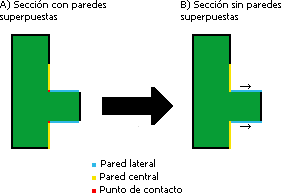
\includegraphics[width=10.5cm, height=7cm]{imagenes/Wall_Overlapping.png}
\caption{Solución al problema de superposición de paredes. (A) Sección con paredes superpuestas. (B) Sección sin paredes superpuestas}
\label{fig:Wall_Overlapping}
\end{figure}

En resumen, la renderización de las secciones del laberinto se genera en 3 pasos:

\begin{itemize}
    \item 1. Renderización del pasillo principal y el portal de entrada a la sección si lo hubiese.
    \item 2. Renderización de los pasillos laterales izquierdos y sus respectivos portales de salida si los hubiese.
    \item 3. Renderización de los pasillos laterales derechos y sus respectivos portales de salida si los hubiese.
\end{itemize}

Cabe añadir que el orden de los pasos 2 y 3 es intercambiable, ya que el procedimiento que se sigue para renderizar los pasillos laterales es prácticamente el mismo independientemente de su orientación y lo único que cambia es el orden en el que se crean.

La clase GraphNode también proporciona métodos para conectar los nodos del grafo, tanto los caminos principales como las ramificaciones. Se debe tener en cuenta que para interconectar los portales de las secciones es imprescindible que dichas secciones se encuentren renderizadas ya que, si no lo están, los portales no existen en primer lugar. 

Tras este proceso, es posible renderizar un nodo en cualquier momento. No obstante, también es necesario poder desrenderizarlo para cumplir con los objetivos del proyecto. Para conseguirlo se ha utilizado la API de Unity, de manera que se destruye el objeto padre que contiene todos los objetos que se han renderizado para dar forma a la sección, destruyendo estos últimos en el proceso. Aunque se ha destruido por completo el objeto, si es necesario volver a renderizarlo es posible hacerlo ya que todos los datos necesarios siguen almacenados en la estructura de datos.

En resumen, gracias a los métodos que permiten la renderización y desrenderización de los nodos y a la estructura de datos en general, la clase GraphNode permite almacenar toda la información sobre las secciones del laberinto y manipular su renderización completamente. Así, sin importar cuantas veces el usuario avance o vuelva atrás en el laberinto, la información de las secciones será la misma y, por lo tanto, los objetos que se crean al renderizarlas también. Esta será una de las clases más importantes a la hora de diseñar el algoritmo de generación del laberinto que se explica a continuación.

\subsection{Algoritmo procedimental de generación de laberintos}

Gracias a la estructura de datos que se ha explicado anteriormente, es posible generar secciones del laberinto con las características que sean necesarias. En este apartado, se explica cómo se hace uso de esta estructura de datos para generar laberintos de forma procedimental con las dimensiones deseadas.

Uno de los principales objetivos del proyecto es que esta generación procedimental tenga en cuenta el espacio de trabajo del usuario, de manera que sea imposible que este se salga y colisione con paredes u objetos del mundo real (Ver figura \ref{fig:Workspace_Example}). Para conseguir esto se define antes de generar el laberinto las dimensiones de la habitación, información que se tiene en cuenta posteriormente. Es importante saber que, cuanto menor sea el espacio de trabajo, menor es la aleatoriedad de los laberintos generados, ya que para producir secciones determinadas se tienen que cumplir ciertas condiciones.

\begin{figure}[h!]
\centering
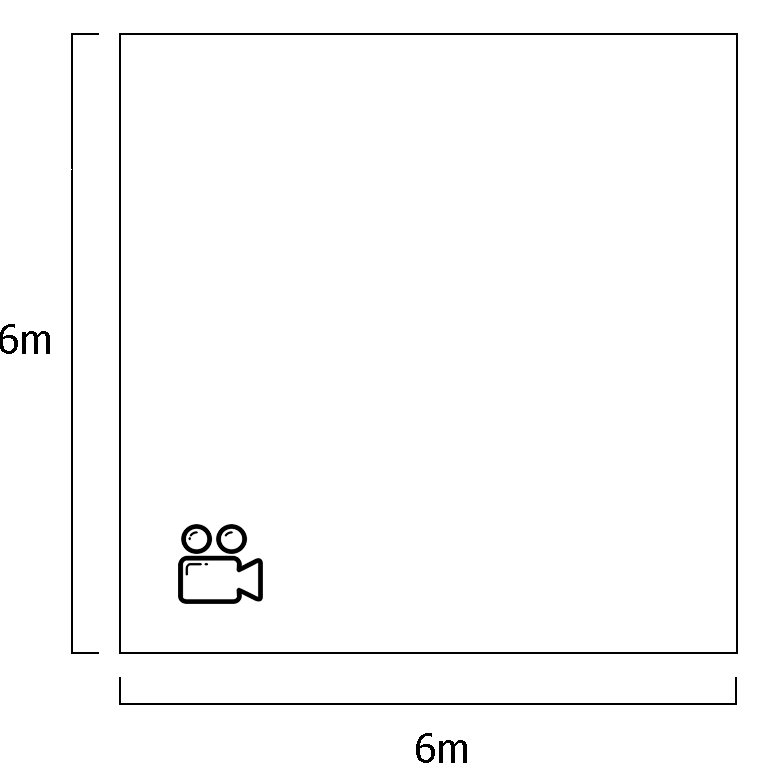
\includegraphics[width=8.5cm, height=8cm]{imagenes/Workspace_Example.png}
\caption{Ejemplo de espacio de trabajo de $6m^2$.}
\label{fig:Workspace_Example}
\end{figure}

Además de las dimensiones del espacio de trabajo, es necesario saber antes de generar una nueva sección las coordenadas actuales del usuario (x,y), actualizando este dato cada vez que se termine de generar una sección, y dependiendo del camino que el usuario tome. Esta información es clave ya que determina por completo el rango de posibilidades de secciones que se pueden crear en determinados momentos. Las coordenadas del usuario, al comienzo de la generación, equivalen al punto del espacio en el que comienza, que debe estar dentro del espacio de trabajo.

Para conseguir tener las coordenadas correctas en todo momento, el espacio de trabajo se trata como una matriz de dimensiones MxN, donde M es el largo de la habitación, y N el ancho. Por ejemplo, en la figura \ref{fig:Workspace_Example} el espacio de trabajo sería una matriz de 6x6 metros, donde el usuario comienza en la esquina inferior izquierda, que corresponde a las coordenadas (1,1).


\begin{figure}[h!]
\centering
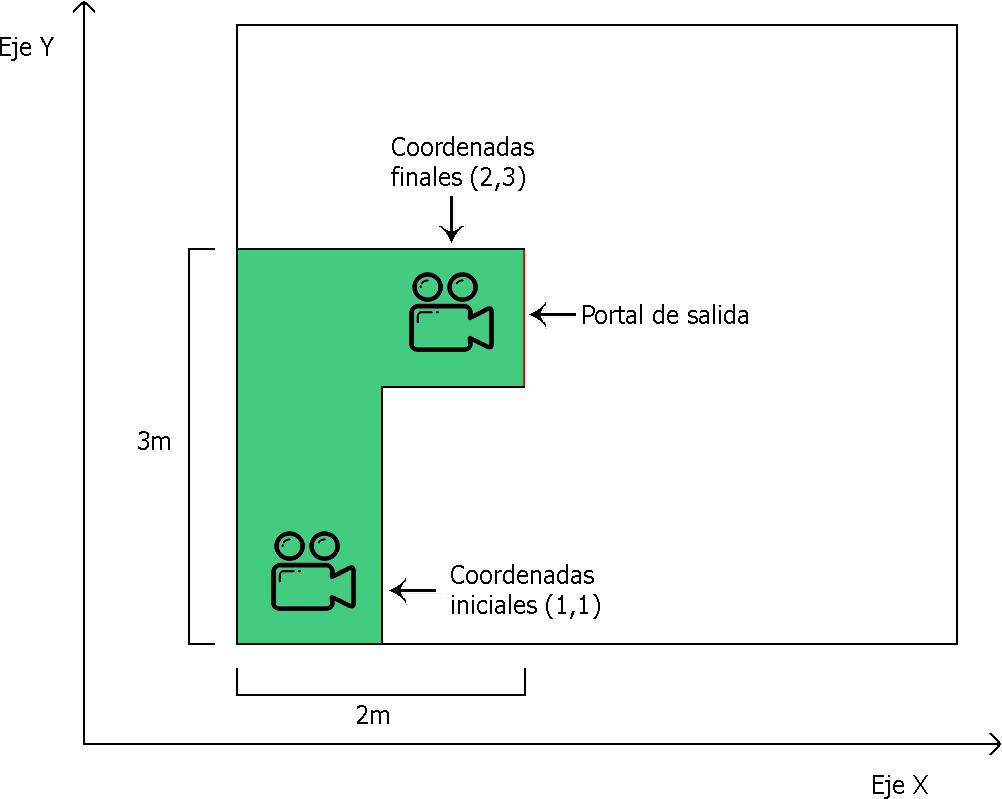
\includegraphics[width=11cm, height=9cm]{imagenes/Coordinates_Update_Example.png}
\caption{Ejemplo de actualización de las coordenadas del usuario cuando la dirección de la sección es hacia arriba y el giro hacia la derecha.}
\label{fig:Coordinates_Update_Example}
\end{figure}

Al terminar de generar una sección, las coordenadas que se busca conseguir al actualizar equivalen al punto en el que termina el pasillo lateral por el que sale el usuario a la siguiente sección. Esto es así para que la siguiente sección pueda crearse en base a esta información. Los pasillos principales de las secciones tienen 4 posibles direcciones, hacia arriba, hacia abajo, hacia la izquierda y hacia la derecha. En todos los casos, primero se guardan dos variables (x,y), siendo x la longitud del pasillo lateral y siendo y el punto del pasillo principal en el que se instancia el pasillo lateral. Se debe tener esto en cuenta ya que el pasillo lateral no tiene por qué crearse al final. Dependiendo de la dirección y del giro que se haya realizado, los cálculos que se realizan para actualizar las coordenadas son diferentes. 

El caso más sencillo es en el que la dirección del pasillo principal es hacia arriba (Ver figura \ref{fig:Coordinates_Update_Example}), ya que simplemente es necesario sumar en la componente Y de las coordenadas el número de metros del pasillo principal hasta llegar al pasillo lateral, y en la componente X sumar o restar, dependiendo de si el giro es a la izquierda o a la derecha, la longitud del pasillo lateral.

En el ejemplo, el usuario empieza en las coordenadas (1,1) de la habitación, y la primera sección generada está compuesta por un pasillo principal de 3 metros y un pasillo lateral derecho al final de este de 1 metro de longitud. Para actualizar las coordenadas del usuario, se ha aumentado la componente X en 3 y a la componente Y en 1. Al ser esta la primera sección, se debe restar 1 a la longitud del pasillo principal, ya que ya se tiene en cuenta en las coordenadas iniciales. De esta forma, se pasa de las coordenadas iniciales (1,1) a las coordenadas finales (2,3), lo que significa que la sección por la que sale el usuario termina tras avanzar 3 metros hacia delante y dos metros a la derecha.

Sin embargo, también existen los nodos en F y T, en los que hay 2 pasillos laterales. En estos casos, se elige aleatoriamente uno de los dos pasillos, que pasa a ser pasillo principal. Esto significa que este pasillo es el que sigue por el camino principal que se estaba creando, y el otro pasillo lleva a una nueva ramificación que debe crearse posteriormente. Por lo tanto, disponemos de dos coordenadas que llevan a dos caminos diferentes (Ver figura \ref{fig:Coordinates_Update_Ramification}).

\begin{figure}[h!]
\centering
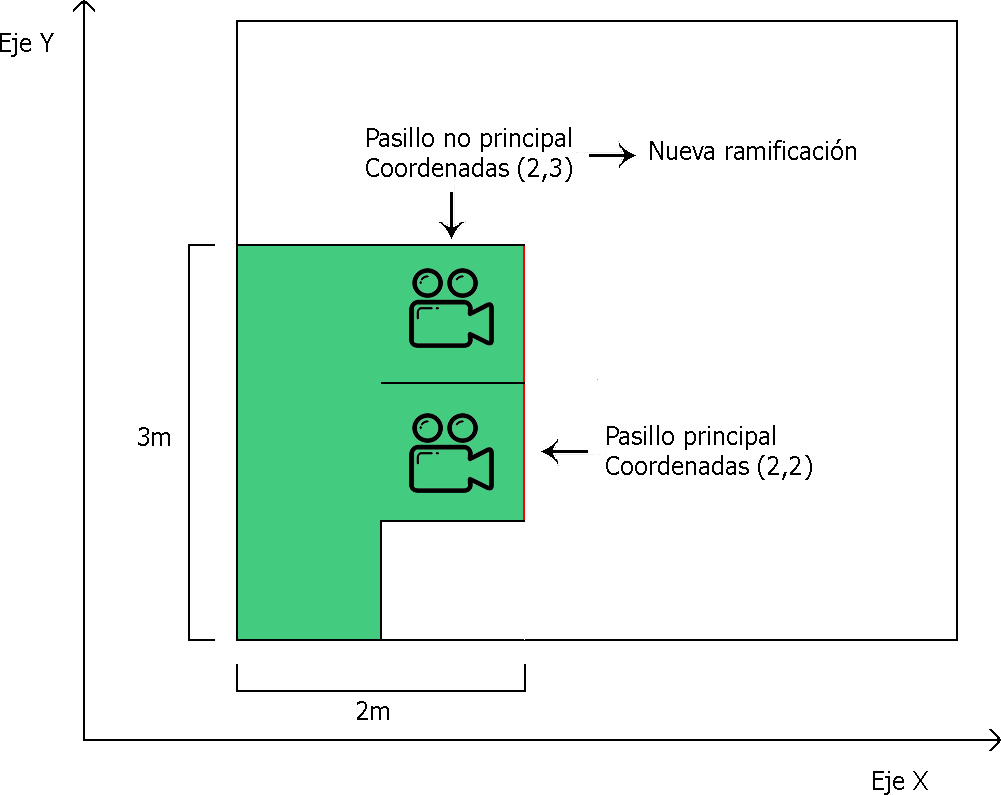
\includegraphics[width=11cm,height=9cm]{imagenes/Coordinates_Update_Ramification.png}
\caption{Ejemplo de actualización de coordenadas cuando la sección generada crea una nueva ramificación.}
\label{fig:Coordinates_Update_Ramification}
\end{figure}


Tras elegir el pasillo principal, se ajustan las coordenadas al no principal, y se crea recursivamente la ramificación a partir de dichas coordenadas. Después, se actualizan las coordenadas de nuevo al pasillo principal, y se sigue el mismo proceso.

Cuando la dirección del nodo es diferente, es necesario actualizar las coordenadas de maneras distintas para que sigan siendo correctas dentro del espacio.

\begin{figure}[!p]
\hspace{-1.75cm}
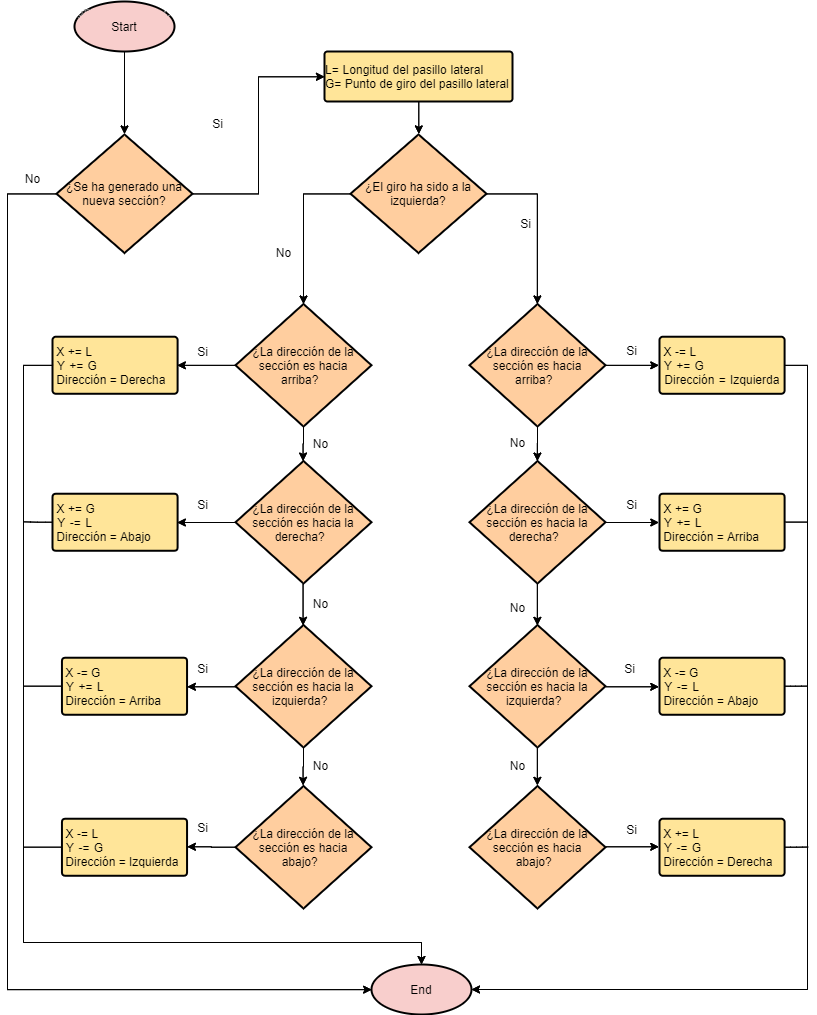
\includegraphics[width=1.3\textwidth]{imagenes/Coordinate_System_Flowchart.png}
\caption{Diagrama de flujo de la actualización de las coordenadas dependiendo de su dirección y el giro realizado.}
\label{fig:Coordinates_Update_System}
\end{figure}

Además de las coordenadas, dependiendo del giro realizado, también hay que actualizar la dirección del nodo, para que la siguiente sección se cree correctamente. Por lo tanto, como se ve en las figura \ref{fig:Coordinates_Update_System}, hay 8 posibles casos base para la actualización de coordenadas.

La lógica que se sigue es simplemente sumar o restar las componentes x e y de las coordenadas según la dirección actual y el giro, para adaptarlas al eje global (x,y) que se puede ver en las figuras \ref{fig:Coordinates_Update_Example} y \ref{fig:Coordinates_Update_Ramification}. Con este sistema, sin importar las características de la sección, siempre se actualizan las coordenadas correctamente.

En cuanto a la posición de las secciones en la escena, como estas están totalmente cerradas por paredes y techos y conectadas por portales, para el usuario es irrelevante donde se encuentren, mientras estén conectadas correctamente y no se encuentren superpuestas, ya que el efecto hace que parezca que están contiguas. Por esto se ha definido un \textit{offset} que determina los metros que se separan lateralmente las secciones en el eje de las X.

También se ha definido otro offset que separa las secciones verticalmente cuando se crea una nueva ramificación, de forma que dicha ramificación comienza donde comenzó el camino principal, pero desplazada en el eje Z (Verticalmente). Estos \textit{offset} deben ser suficientemente grandes para asegurar que las secciones no se solapen unas con otras.

Después de este proceso se dispone de un sistema que actualiza las coordenadas del jugador, dependiendo del camino que tome, para generar las siguientes secciones y ramificaciones del laberinto.

Durante el diseño de este algoritmo se han detectado multitud de condiciones que determinan las características y los tipos de secciones que es posible crear. Para comprender estas condiciones, es necesario entender primero que, debido a las características del espacio, si no se puede girar hacia un lado, siempre se puede girar hacia el otro. Esta información es clave ya que permite asegurar que siempre se puede crear una sección nueva que tenga entrada y salida.

Las condiciones más importantes que definen las características de las secciones son las siguientes:

\begin{itemize}
    \item Es posible girar a la izquierda
    \item Es posible girar a la derecha
    \item Es posible girar hacia ambos lados
\end{itemize}

A partir de estas condiciones se decide siempre con la mayor aleatoriedad posible la forma de la sección y sus características(Ver figura \ref{fig:Decision_Flowchart}).

Siguiendo esta lógica, después de actualizar las coordenadas y siempre que aún no se haya terminado de construir el laberinto, se genera una nueva sección. En el caso de las ramificaciones, se crean 2 procesos de generación de secciones mientras que para las secciones en L se genera uno solo.

Como se ha mencionado anteriormente, siempre es posible realizar un giro hacia una dirección, por lo que es un hecho que sea cual sea la longitud del laberinto y siempre y cuando las características de las secciones sean correctas será posible construir el laberinto.

\begin{figure}[!p]
\hspace{-1.75cm}
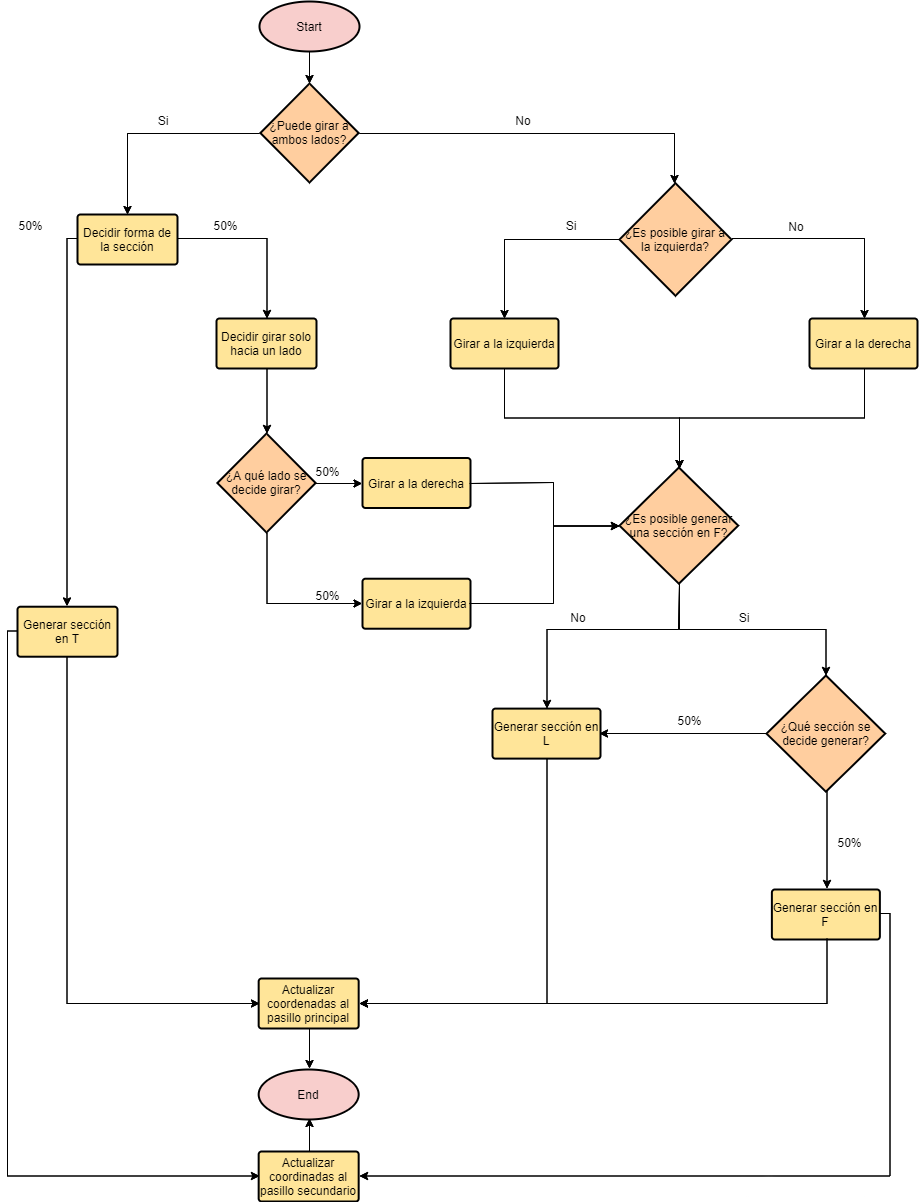
\includegraphics[width=1.3\textwidth]{imagenes/Diagrama_de_Flujo.png}
\caption{Diagrama de Flujo de la generación de las secciones del laberinto.}
\label{fig:Decision_Flowchart}
\vspace{-78.96pt}
\end{figure}

El procedimiento que se utiliza busca siempre que tanto las secciones como el laberinto en conjunto sean lo más variados posibles. Un  ejemplo de esto se puede ver cuando se cumple la condición que comprueba si es posible hacer un giro en ambos sentidos ya que, aunque la condición se cumpla, no se genera directamente una sección en T que gira a ambos lados, sino que hay un 50\% de probabilidad de que se genere el giro hacia un solo lado y, dentro de dicho giro, es igual de probable que gire a la derecha o a la izquierda.

Si esto no fuese así, dada la limitación existente en el espacio de trabajo del usuario, podrían darse casos en los que las secciones y las direcciones y giros de estas fuesen muy similares y, por lo tanto, la sensación de aleatoriedad desapareciese.

Las dimensiones y características de las secciones generadas en el algoritmo procedimental siempre se crean tras  haber  definido  qué  tipo  de  secciones  es  posible  generar  dependiendo  de las condiciones del espacio en determinados puntos, es decir, primero es necesario decidir la forma de la sección y la dirección del giro.

Cada vez que se genera una nueva sección se comprueban los giros posibles que se pueden hacer. Como las secciones están conectadas por portales, los pasillos laterales que se juntan con la nueva sección forman un nuevo pasillo, que tiene que tener una longitud máxima para cumplir con las restricciones del espacio de trabajo.

Para facilitar la generación, los pasillos laterales que se crean son siempre de 1 metro de longitud. De esta forma es suficiente con controlar la longitud de los pasillos principales de las nuevas secciones para asegurar que el laberinto sigue dentro de los límites. 

\begin{figure}[h!]
\centering
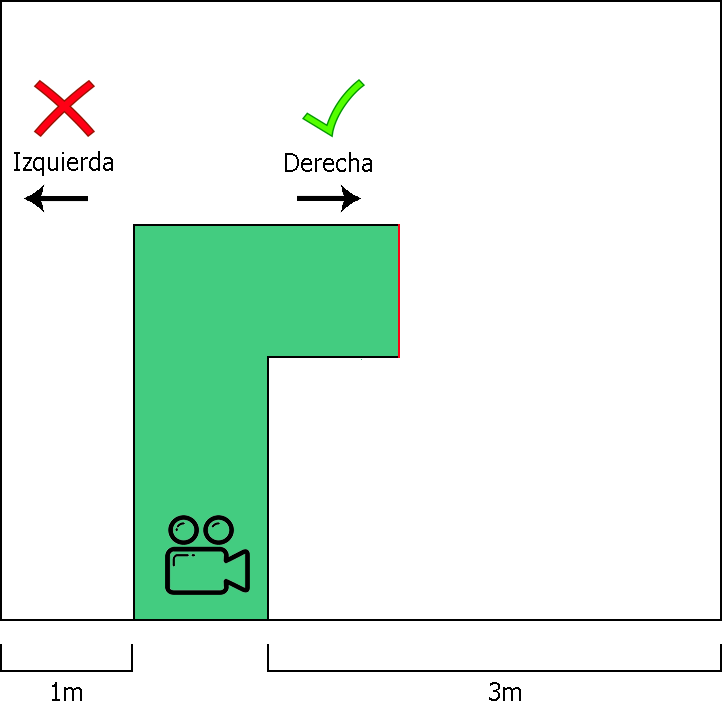
\includegraphics[width=8cm,height=8cm]{imagenes/Turn_Decision.png}
\caption{Ejemplo de comprobación de los posibles giros para una sección.}
\label{fig:Turn_Decision}
\end{figure}

La longitud mínima de los pasillos principales debe ser de 2 metros. Esto es así para evitar que el usuario pueda visualizar portales que aún no están conectados dado que su sección siguiente aún no ha sido renderizada. Para comprobar qué giros se pueden hacer, se comprueba si al girar en dicha dirección, como mínimo, hay una distancia de 3 metros hasta el final. Si se cumple esta condición siempre es posible generar una nueva sección que gire en esa dirección ya que deja espacio suficiente para generar otra nueva. 

En la figura \ref{fig:Turn_Decision} se ve un ejemplo del proceso que se sigue. Se comprueba el espacio disponible hacia la izquierda, que es 1 metro, por lo que el giro a la izquierda es imposible. Después, se comprueba el espacio a la derecha, que es de 3 metros y por lo tanto la sección crea un giro hacia la derecha en un punto del pasillo principal aleatorio.

La sección resultante puede ser, en este caso, tanto en forma de L como F, dependiendo de la longitud del pasillo principal. Al ser los polígonos de $1m^2$, una sección en forma de F solo es posible cuando la longitud del pasillo principal es mayor o igual a 3 metros. Para los pasillos en forma de T la longitud del pasillo principal debe ser igual o mayor a 4 metros, dadas las restricciones existentes.

Una vez explicadas todas las condiciones y posibilidades, finalmente se puede generar el pasillo principal, que condiciona la forma de la sección. 

Como se explica anteriormente, la su longitud mínima siempre es 2 metros, pero la máxima depende de varios factores. Este valor depende en gran medida del tamaño del espacio de trabajo disponible por el usuario, es decir, cuanto mayor sea el espacio de trabajo, más posibilidades de generar pasillos principales de mayor longitud hay.

Otro factor que determina su longitud es la dirección de la sección, ya que define la dirección del espacio de trabajo en la que se calcula el espacio disponible. De esta forma, se genera una longitud aleatoria de entre un mínimo de 2 metros y un máximo que será igual a la distancia que hay desde la posición en la que se encuentre la sección, hasta el límite del espacio de trabajo en la dirección de la sección.

Para hacer este cálculo se ha seguido un procedimiento muy similar al que se sigue en la actualización de coordenadas (Ver figura \ref{fig:Coordinates_Update_System}), pero en vez de actualizar las coordenadas, se miran los valores en función de la dirección.

Siguiendo este procedimiento se asegura que las secciones están siempre dentro de los límites del espacio de trabajo y, al estar conectados los pasillos laterales con los principales, solo es necesario controlar la longitud de estos últimos, ya que siempre se deja espacio para secciones nuevas.

La longitud del pasillo principal es lo primero que se genera al comenzar una nueva sección, ya que su forma o el punto donde gira dependen de esta.

Por ejemplo, en la figura \ref{fig:Straight_Hallway_Generation}, en un espacio de trabajo de 5 metros de ancho y largo, la sección actual termina en las coordenadas (3,4). La dirección de dicha sección es hacia la derecha, y el giro también, por lo que la dirección de la nueva sección a generar es hacia abajo.

Sabiendo esto, en este caso la distancia disponible es igual a la componente Y de las coordenadas del jugador, restándole 1 metro, es decir $4-1 = 3$ metros. El pasillo principal puede tener cualquier longitud en este rango, ya que al generar los pasillos laterales siempre se asegura que existe espacio para una nueva sección. Por lo tanto el pasillo generado será de 2 o 3 metros.

\begin{figure}[h!]
\centering
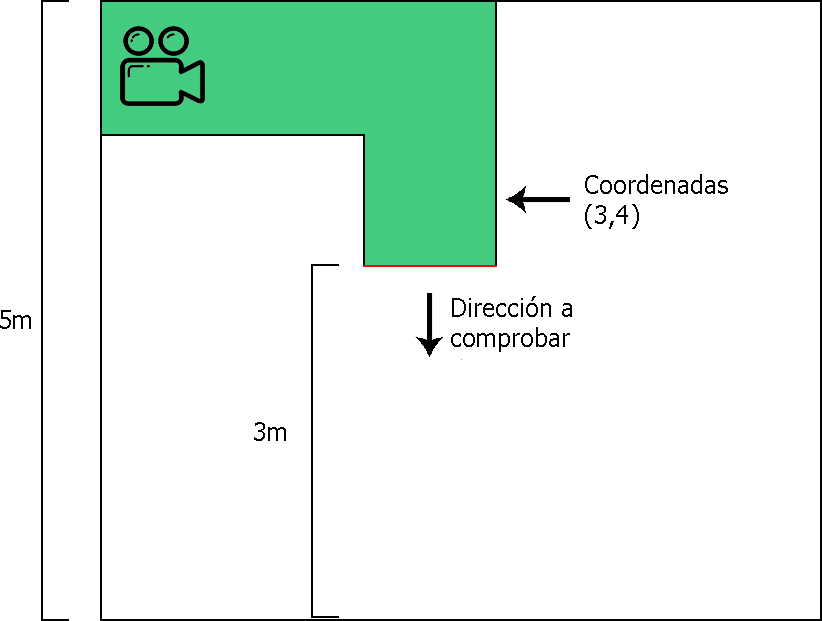
\includegraphics[width=10cm,height=8cm]{imagenes/Straight_Hallway_Generation.png}
\caption{Ejemplo de generación de la longitud de un pasillo principal de una nueva sección.}
\label{fig:Straight_Hallway_Generation}
\end{figure}

Finalmente, para que el usuario pueda ubicarse mejor en el laberinto y sepa cuando ha llegado al final de este, en todas las generaciones se añaden tanto a la primera sección como a la sección final un indicador. Este indicador es simplemente una esfera tridimensional que empieza siendo de color rojo y cambia a verde cuando el usuario colisiona con ella.

Tras todo el proceso, se dispone finalmente de un sistema de generación de laberintos procedimental, separados por secciones interconectadas por unos portales que se pueden atravesar para explorar el entorno. Además, la generación asegura que el usuario que recorre el entorno virtual se encuentra siempre dentro de los límites del espacio de trabajo disponible. Este laberinto queda almacenado en un grafo que es completamente manipulable y del que se puede obtener cualquier información relevante y que permite renderizar las secciones necesarias en cada momento.

Sin embargo, uno de los objetivos del proyecto es renderizar estas secciones dinámicamente, de manera que se mejore el rendimiento aumentando la eficiencia. A continuación se explica el proceso que se ha seguido para conseguirlo y cómo funciona el sistema.

\subsection{Renderización dinámica de las secciones del laberinto}

La estructura de datos que se ha creado previamente para almacenar el laberinto permite un control total sobre este, lo que facilita mucho la renderización dinámica de las secciones.

Antes de explicar cómo funciona es necesario entender la detección de colisiones en Unity, que es la base del sistema. En Unity existen unos componentes llamados Colliders que permiten detectar colisiones con otros objetos de la escena. Cada portal que se renderiza tiene uno de estos componentes que lo envuelve, de forma que cuando un ojo colisiona con uno de los portales, se teletransporta al portal conectado.

Para asegurar que se sabe en todo momento en que sección se encuentra el jugador, se le ha añadido a uno de los ojos del objeto XR Rig un Collider y un Script, que detecta únicamente las colisiones de este con los portales. Esto es necesario porque son los ojos los que se teletransportan, no el objeto en sí. De esta manera sabemos en qué momento el usuario está cruzando un portal.

No obstante, hay que diferenciar si el portal con el que se colisiona es de entrada o de salida, ya que la sección a la que se teletransporta al usuario es distinta y, por lo tanto, las secciones que se deben renderizar también. Esto se ha conseguido fácilmente accediendo al nombre del objeto que contiene el portal.

Si el usuario cruza un portal de salida, significa que está avanzando hacia delante en el laberinto, mientras que si cruza un portal de entrada, significa que está avanzando hacia atrás. Ambos casos deben estar contemplados y bien distinguidos para la correcta renderización de las secciones.

\begin{figure}[h!]
\centering
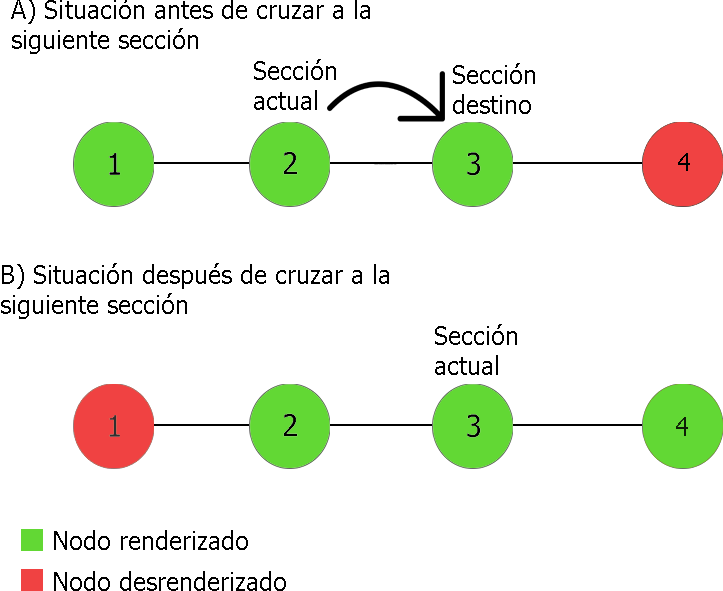
\includegraphics[width=10.5cm,height=8.5cm]{imagenes/Simple_Node_Render_Case.png}
\caption{Ejemplo de renderización dinámica de secciones cuando la sección actual es en forma de L. A) Situación antes de cruzar la siguiente sección. B) Situación después de cruzar a la siguiente sección.}
\label{fig:Simple_Node_Render_Case}
\end{figure}

Una vez se pueden detectar las colisiones y sobre qué tipos de portales ocurren, hay que definir qué secciones se deben renderizar y cuáles no. Si la colisión que se detecta es con una sección de salida, hay 2 casos posibles:

\begin{itemize}
    \item La sección actual es en forma de L.
    \item La sección actual es en forma de T o F.
\end{itemize}

El primer caso es el más sencillo, ya que si la sección tiene forma de L solo existe un único portal de salida y no existen ramificaciones. Una vez detectada la colisión, se renderizan todas las secciones que estén conectadas con la sección destino del usuario (Ver figura \ref{fig:Simple_Node_Render_Case}). Si la sección destino tiene forma de T o F, se renderizan varias secciones, mientras que si es en L solo es necesario renderizar una. También se  deben desrenderizar todas las secciones conectadas con la sección anterior a la actual, ya que no son necesarias a partir de este momento. Finalmente se actualiza la sección actual para preparar el sistema para la siguiente colisión.

Siguiendo este proceso se asegura que solo están renderizadas en la escena las secciones necesarias. El número de secciones que están renderizadas en cualquier momento debe ser siempre igual a 1, correspondiente a la sección actual, más el número de portales que tenga dicha sección. 

Si la sección es en L, el número de secciones renderizadas siempre es 3, mientras que si es en F o T, debe renderizarse una sección por cada pasillo lateral abierto que la sección tenga, además de la anterior. Lo mismo pasa en la desrenderización, si la sección anterior a la actual tiene ramificaciones, deben desrenderizarse todas las secciones que tenga conectadas, además de ella misma.

El segundo caso no es tan sencillo ya que la sección actual tiene varios portales de salida, por lo que también es necesario diferenciar cuál de los portales de salida es colisionado para saber qué camino a tomado el usuario y renderizar las secciones de forma coherente.

Para poder diferenciar los caminos, se accede al portal con el que se ha colisionado y se comprueba si el pasillo al que pertenece lleva por el camino principal o a una ramificación. Si el portal lleva por el camino principal, se procede como se ve en la figura \ref{fig:Simple_Node_Render_Case}, y si lleva a una nueva ramificación se actualiza la sección al primer nodo de la ramificación y se renderizan sus secciones conectadas. Finalmente, igual que en el resto de casos, se desrenderizan las secciones conectadas a la sección anterior a la actual, ya que en este punto no son necesarias.

Aunque todas las secciones tienen un único portal de entrada, cuando se detecta una colisión con ellos también existen 2 casos posibles:

\begin{itemize}
    \item La sección actual y la sección anterior pertenecen a la misma ramificación o al camino principal.
    \item La sección actual y la sección anterior pertenecen a ramificaciones distintas.
\end{itemize}

El primer caso es muy similar al que se ve en la figura \ref{fig:Simple_Node_Render_Case}, pero la dirección en la que se avanza es la opuesta. Cuando se detecta la colisión se renderizan las secciones conectadas a la sección anterior y se desrenderizan las secciones conectadas a la sección siguiente. Por último se actualiza la sección actual.

Si ocurre el segundo caso significa que la sección actual, sobre la que se ha detectado una colisión con un portal de entrada, es la primera sección de una ramificación. Esto supone un problema, ya que no existe una sección previa a esta al ser la primera de su ramificación. Para poder actualizar los nodos correctamente, se busca la conexión que une la sección actual a la sección que creó la ramificación. 

\begin{figure}[h!]
\centering
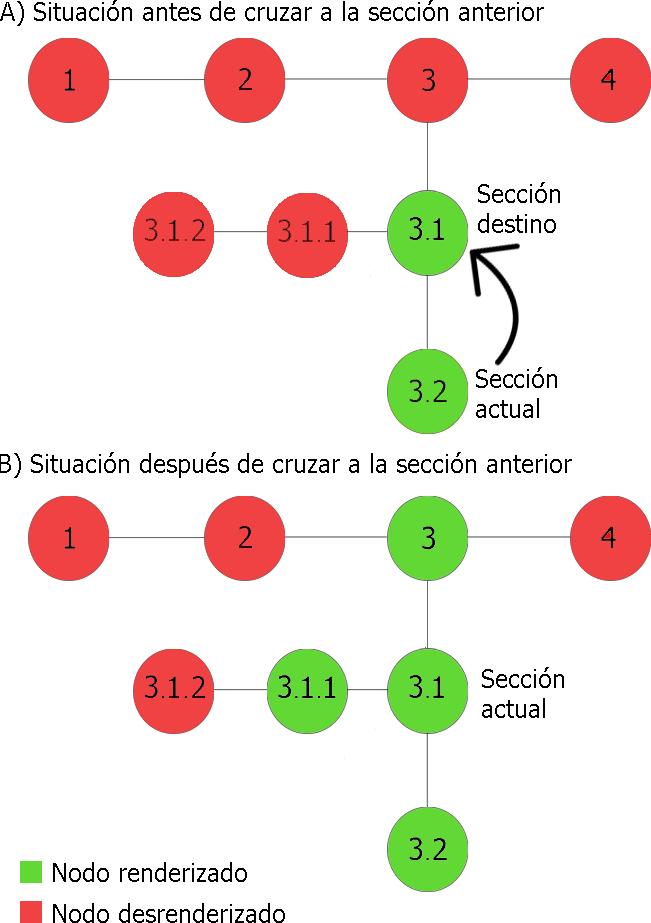
\includegraphics[width=10.5cm,height=13.5cm]{imagenes/Entry_Portal_Render.png}
\caption{Ejemplo de renderización dinámica de secciones cuando la sección actual y la anterior pertenecen a ramificaciones diferentes. A) Situación antes de cruzar a la sección anterior. B) Situación después de cruzar a la sección anterior.}
\label{fig:Entry_Portal_Render_Case}
\end{figure}

Como se ve en la figura \ref{fig:Entry_Portal_Render_Case}, una vez se tiene la referencia a dicha sección se sigue el mismo proceso que en el resto de casos. Primero se desrenderizan las secciones conectadas a la sección actual y después se renderizan las secciones conectadas a la sección que creó la ramificación, que pasa a ser la actual. En la situación que se muestra antes de cruzar a la sección anterior solo se encuentran renderizadas 2 secciones, puesto que la sección actual es la última de esa ramificación, y solo tiene 1 sección conectada, mientras que tras cruzar hay 4 secciones renderizadas.

Además de las paredes, techos, suelos y portales, también se deben renderizar los indicadores de inicio y final del laberinto. Como se menciona antes, estos son esferas que cambian de rojo a verde cuando el usuario colisiona con ellas. Para preservar su estado, se guarda en la estructura de datos si el usuario ha colisionado previamente con el indicador o no.

Si ha colisionado previamente, al renderizar el indicador debe hacerse directamente con el color en verde, mientras que si no lo ha hecho, debe renderizarse en su estado inicial, con el color en rojo.

Para asegurar que el sistema de renderización dinámica establece correctamente la sección en la que se encuentra el usuario en todo momento, es necesario controlar algunos aspectos de la colisión con los portales. El principal problema que surge es que, al teletransportar los ojos de una sección a otra, también se teletransporta su componente collider, por lo que Unity detecta la colisión con el portal de entrada instantáneamente en el momento del teletransporte.

Antes de explicar la solución a este problema, es necesario recordar cómo funciona el teletransporte entre portales. Como se explica en la sección \ref{Unity_Portals}, se detectan las colisiones de cada ojo por separado, para permitir que el usuario pueda hacer acciones como introducir la mitad del cuerpo dentro del portal, dejando la otra mitad al otro lado. Para conseguir esto, se utiliza una pequeña distancia llamada offset de manera que si el ojo se encuentra a esa distancia del portal, se teletransporta al otro lado. 

Para evitar que se detecten colisiones en el instante del teletransporte, el collider que se ha creado tiene un grosor menor que el offset que se utiliza en el teletransporte. Gracias a esto nos aseguramos de que para que se detecte una colisión, el usuario siempre tiene que andar hacia uno de los portales. La altura de este collider también debe ser mínima porque si el usuario mira hacia abajo podría hacer colisionar el collider con un portal, ya que este es hijo del objeto padre en Unity.

Detectando las colisiones correctamente y teniendo en cuenta la forma y posición de los nodos que forman el grafo, siguiendo este proceso se puede renderizar dinámicamente cualquier laberinto generado, de forma que siempre es el mismo, todas las secciones pueden ser visitadas un número ilimitado de veces, y solo se renderizan simultáneamente las que son completamente necesarias.

\end{document}